% 第41回情報理論とその応用シンポジウム 予稿集 原稿様式
% pTeX, Version p3.1.3, based on TeX, Version 3.141592 (sjis) (Web2C 7.5.2)
% 本文: 日本語

\documentclass{jarticle}
\usepackage{sita2018,amsmath,amssymb,amsfonts}
\usepackage[dvipdfmx]{graphicx}
\title{
  近似的メッセージ伝播法に基づくパイロット汚染の軽減 \\
  Reduction of pilot contamination based on approximate message passing
}
%
\author{
藤塚 拓実
  \thanks{ 
    〒441-8580 愛知県豊橋市天伯町雲雀ヶ丘1-1 豊橋技術科学大学 電気・電子情報工学専攻 通信信号処理研究室 Communication \& Signal Processing Lab., Department of Electrical and Electronic Information Engineering, Toyohashi University of Technology
    E-mail: {\tt fujitsuka@\allowbreak
    comm.\allowbreak
    ee.\allowbreak
    tut.\allowbreak
    ac.\allowbreak
    jp}
  }\\
  Fujitsuka Takumi
%
  \and
竹内 啓悟
% %第二著者名(和文)
\thanks{
    \samethanks{1} 
% %第二著者の所属と住所(和文と英文)
% %もし第一著者と同じならば,\thanks{}の代りに\samethanks{1}を使ってください.
  }\\
% %第二著者名(英文)
Takeuchi Keigo
}

\abstract{
%英文のアブストラクト
Practical application of fifth generation wireless communication (5G) is being promoted with the goal of 2020. Massive MIMO is the most important technique in 5G. 
Massive MIMO optimizes communication for each terminal by performing beamforming on the downlink. It is necessary to obtain channel state information (CSI). CSI is estimated by transmitting a known signal called a pilot signal transmitted by the user to the base station on the uplink. When estimating CSI in that way, a phenomenon called pilot contamination, which is interference between base stations, occurs. In this research, we aim to mitigate pilot contamination in uplink massive MIMO system. For that purpose, we aim to simultaneously estimate CSI and data using the Approximate Message Passing (AMP) after shifting the transmission timing of the pilot by time for each base station. In the research until last year there was a difficulty in convergence of AMP, but by using early change of algorithm and damping, we improved convergence.
}
\keywords{
 Massive MIMO, pilot contamination, Approximate Message Passing(AMP), compressed sensing
}
  
\begin{document}
\maketitle

\section{はじめに}
移動通信の標準化団体3GPPや総務省,企業,大学などが連携し,国内外で2020年を目標として第5世代無線通信(5G)の標準化が推進されている\cite{5gmf}.5Gにおける最も重要な技術として大規模MIMO(Massive MIMO)\cite{Marzetta}\cite{Rusek}がある.大規模MIMOでは基地局からユーザにデータを送信するダウンリンクにおいて,ビームフォーミングを行うことで端末ごとの通信を最適化するが,そのためには通信路状態情報(Channel State information : CSI)を得る必要がある.CSIを得る方法として,ユーザが基地局にデータを送信するアップリンクにおいて,ユーザがパイロット信号と呼ばれる既知信号を基地局に送信することでCSIを推定する方法がある.しかし,コヒーレンス時間によってパイロット信号の長さが制限されるため,隣接する基地局と同一のパイロット信号を使用することになり,同一のパイロット信号することでCSIの推定が困難になる現象をパイロット汚染\cite{Marzetta}と呼ぶ.

パイロット汚染を軽減する方法として,基地局ごとにパイロットの送信タイミングを時間シフトさせて送信する手法が提案されている\cite{Appaiah}.本研究では,パイロット信号を基地局で時間シフトさせた上で,復号アルゴリズムとして樺島が定式化した近似的メッセージ伝播法(Approximate Message Passing :AMP)\cite{kabashima}を使用する手法を提案する.提案した手法を数値シミュレーションによって有用性を比較・検証する.

\section{システムモデル}
複数のセルが隣接し,各セルが複数のユーザとアンテナを有し(MU-MIMO),ユーザがセルにデータを送信するアップリンクを想定する.隣接セル数を$L$とし,$L=1$のセルは他の$L-1$のセルのユーザから干渉を受ける.$T$シンボル送信し,各セルのユーザ数を$K_{l}$,受信アンテナ数を$N$とし,ユーザは単一の送信アンテナを持つことを想定する.また,簡単のため,フェーディング係数は$T$の間一定であるブロックフェーディング通信路を仮定する.受信ベクトル$\boldsymbol{y}_t \in \mathbb{C}^{N}$は(\ref{eq:sys})式にて与えられる.($t \in {1,...,T}$)
\begin{equation}
    \label{eq:sys}
    \boldsymbol{y}_t = \boldsymbol{H}[1]\boldsymbol{x}_{t}[1]+\sum^{L}_{l=2}\boldsymbol{H}[l]\boldsymbol{x}_{t}[l]+\boldsymbol{w}_{t}.
\end{equation}
$\boldsymbol{H}[1]\in\mathbb{C}^{N\times K_{1}}$は自セルのユーザとアンテナ間のフェーディング係数であり通信路行列(CSI)である.$\boldsymbol{H}[l]\in\mathbb{C}^{N\times K_{l}} ,l \in {2,...,L}$は隣接セルのユーザとアンテナ間のフェーディング係数であり,干渉ユーザに相当する.ここで,$\boldsymbol{H}$に関して,すべての行列成分は,互いに独立で同一の分布(independent and identically distribution : i.i.d)のレイリーフェーディングに従うと仮定する.具体的には,それぞれが独立した円対称複素ガウス雑音(Circularly Symmetric Complex Gaussian : CSCG)であり,分散は$1/N$とした.また,$\boldsymbol{w}_{t}\in\mathbb{C}^{N}$は受信時に生じる雑音であり,それぞれが独立した円対称複素ガウス雑音で,分散は定数$N_0$とした.

(\ref{eq:sys})式を行列式で表すため,$\boldsymbol{Y}=(\boldsymbol{y}_{1},...\boldsymbol{y}_{T})\in\mathbb{C}^{N\times T},\boldsymbol{W}=(\boldsymbol{w}_{1},...\boldsymbol{w}_{T})\in\mathbb{C}^{N\times T}\boldsymbol{H}=(H[1],..,,H[L])\in\mathbb{C}^{N\times K}(K=\sum_{l=1}^{L}K_l),\boldsymbol{X}=(X^{T}[1],...,X^{T}[L])^T\in\mathbb{C}^{K\times T}$と定義すると(\ref{eq:sys})式は(\ref{eq:matsys})式のように書ける.
\begin{equation}
    \label{eq:matsys}
    \boldsymbol{Y} = \boldsymbol{HX+W}
\end{equation}
データシンボル$x_{nt} = [\boldsymbol{X}]_{nt}$は平均電力$P_{n}=\mathbb{E}[|x_{nt}|^{2}]$である.

目標は,時分割複信(Time Division Duplex :TDD)ダウンリンクにおいてビーム形成を実行するために,自セル($l=1$)で全体の通信路行列$\boldsymbol{H}$とデータ$\boldsymbol{X}_1$の推定をすることである.送信シンボルはQPSK信号を送信する.

本研究ではパイロット信号を軽減するために,セル間での協調を必要とする.具体的には,長さ$Tp$パイロット信号の送信タイミングを基地局ごとに時間シフトさせて送信するように制御する.少なくとも$Tp$以上時間を空けて隣接セルのパイロット信号を送信する必要がある.したがってダウンリンクでビームフォーミングを行うためにも$Tp$はできる限り短くする必要がある.

\section{近似的メッセージ伝播法 AMP}
従来の通信路推定は,正確なチャネル推定値を得るために長いパイロットシーケンスを必要とする.本研究ではパイロット信号を短くするため,AMPに基づく通信路とデータの同時推定アルゴリズムを提案する.

近似的メッセージ伝播法は,人口知能分野で提案された確率伝播法(Belief Propagation BP)を基礎として発展した統計学的手法である.もともとは,圧縮センシングの分野で提案された手法である\cite{Donoho}.樺島の手法ではAMPを使って通信路推定とデータ推定を行うことができるよう定式化された\cite{kabashima}.本研究では,通信路($\boldsymbol{H}$)推定部とデータ($\boldsymbol{X}$)推定部に分け,この二つの推定結果を使って,通信路推定とデータ推定を交互に繰り返すことで推定精度を向上させていく.

提案手法では,推定されたデータが追加のパイロットシンボルとして利用されるので,短いパイロット系列で精度の高い推定を可能にする.

通信路推定器とデータ推定器から構成され,各推定器の反復を内部反復,2つの推定器間の反復を外部反復と呼ぶ(図\ref{fig:flow}参照).
\begin{figure}[htbp]
    \begin{center}
     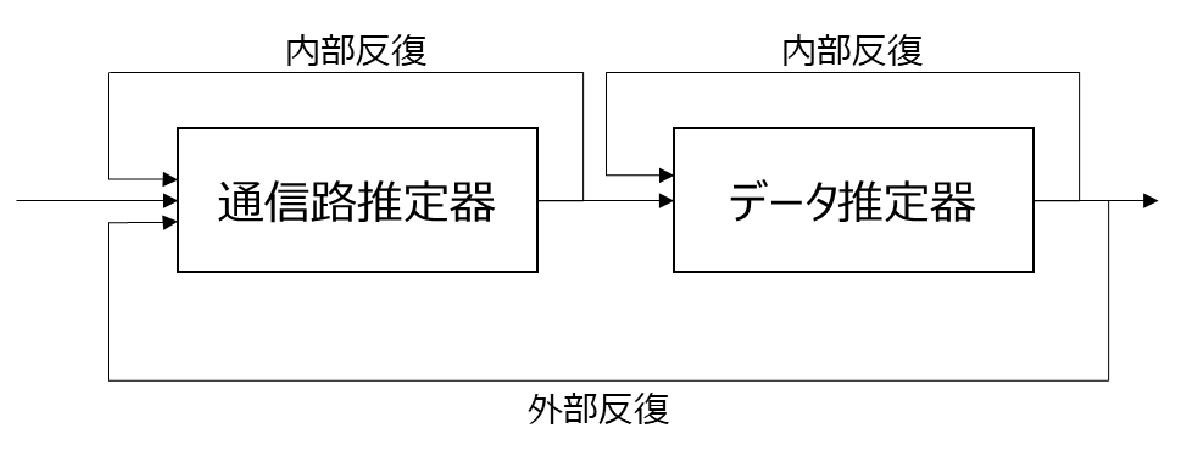
\includegraphics[width=80mm]{./flow.eps}
    \end{center}
    \caption{提案手法の計算順序}
    \label{fig:flow}
\end{figure}

詳細な説明をする前に,いくつかの表記法を定義しておく.$\hat{h}_{nk}\in\mathbb{C},\eta_{nk} >0$はそれぞれ,$h_{nk}=[\boldsymbol{H}]_{nk}$とその平均2乗誤差(MSE)の推定値である.通信路推定に関わるメッセージは${\cal C}=\{\hat{h}_{nk},\eta_{nk}\}$とする.前回の外部反復の通信路推定のメッセージは${\cal C}_{pre}=\{\hat{h}_{nk}^{pre},\eta_{nk}^{pre}\}$とする.同様にデータ推定に関して,$\hat{x}_{kt}\in\mathbb{C},\xi_{kt}>0$はそれぞれ,$x_{kt}=[\boldsymbol{X}]_{kt}$とMSEの推定値である.データ推定に関わるメッセージは${\cal D}=\{\hat{x}_{kt},\xi_{kt}\}$とする.前回の外部反復のデータ推定のメッセージは${\cal D}_{pre}=\{\hat{x}_{nk}^{pre},\xi_{kt}^{pre}\}$とする.

$z_{nt}\in\mathbb{C}$を受信信号$y_{nt}=[\mathbb{Y}]_{nt}$からすべての推定値を減算した残差とする.さらに,$z_{nt}$の平均電力を$\zeta_{nt}$とする.残差信号に関するのメッセージを${\cal R}=\{ z_{nt},\zeta_{nt}\}$とする.通信路推定器とデータ推定器共にメッセージ${\cal R}$を出力するので,それぞれ${\cal R_{c}}=\{ z_{nt}^{c},\zeta_{nt}^{c}\},{\cal R_{d}}=\{ z_{nt}^{d},\zeta_{nt}^{d}\}$と区別する.残差$z_{nt}$は(\ref{eq:residual})式のように表される.
\begin{equation}
    \label{eq:residual}
    \begin{split}
    z_{nt}({\cal C},{\cal C}^{pre},{\cal D},{\cal D}^{pre},{\cal R}_{c},{\cal R}_{d}) = y_{nt} - \sum_{n=1}^{N}\hat{h}_{nk} \hat{x}_{kt} \\
    \quad +\sum_{n=1}^{N}\frac{\eta_{nk}(\hat{x}_{kt}^{pre})^{*}\hat{x}_{kt}z^{c}_{nt}}{\zeta_{nt}^{c}}+\sum_{n=1}^{N}\frac{(\hat{h}_{nk}^{pre})^{*}\hat{h}_{nk}\xi_{kt}z^{d}_{nt}}{\zeta_{nt}^{d}} 
    \end{split}
\end{equation}
また,$\zeta_{nt}$は(\ref{eq:zeta})式のように表される.
\begin{equation}
    \label{eq:zeta}
    \zeta_{nt}({\cal C},{\cal D}) = N_{0} + \sum_{n=1}^{N}\{\eta_{nk}(\xi_{kt}+|\hat{x}_{kt}|^2)+|\hat{h}_{nk}|^2\xi_{kt}\}
\end{equation}
(\ref{eq:residual})(\ref{eq:zeta})式は二つの推定器の両方で計算される.

\subsection{通信路推定}
通信路推定器では,前回の外部反復における,通信路推定器の内部反復の最後で得られた${\cal C}^{pre},{\cal R}_{c}^{pre}$と,データ推定器から得られる${\cal D},{\cal R}_{d}$がある.内部反復変数を$i$とすると,メッセージ${\cal C}_{i},{\cal R}_{i}$は干渉除去のMFフィルタと要素ごとのLMMSEフィルタから構成される.MFフィルタはそれぞれ,(\ref{eq:h_b})(\ref{eq:eta_b})式で表される.
\begin{equation}
    \label{eq:h_b}
    \bar{h}_{nk}^{i} = \hat{h}_{nk} + \bar{\eta}_{nk}\sum_{t=1}^{T}\frac{\hat{x}^{*}_{kt}z^{i}_{nt}}{\zeta_{nt}^{i}} - \bar{\eta}_{nk}\hat{h}^{pre}_{nk}\sum_{t=1}^{T}
    \frac{\xi_{kt}(z^{d}_{nt})^{*}z_{nt}^{i}}
        {\zeta_{nt}^{i}\zeta_{nt}^{d}}
\end{equation}
\begin{equation}
    \label{eq:eta_b}
    \bar{\eta}_{nt}^{i}=  \left(\sum_{t=1}^{T}\frac{|\hat{x}_{kt}|^{2}}{\zeta_{nt}^{i}})\right)^{-1}
\end{equation}
$z^{i}_{nt},\zeta_{nt}^{i}$はそれぞれ,$z^{i}_{nt}({\cal C}_{i},{\cal C}^{pre},{\cal D},{\cal D},{\cal R}_{i-1},{\cal R}_{d}),\zeta_{nt}^{i}({\cal C}_{i},{\cal D})$であり(\ref{eq:residual})(\ref{eq:zeta})式に対応する.

通信路推定の結果$\hat{h}_{nk}^{i+1}$と,そのMSE$\eta_{nk}^{i+1}$は,要素ごとのLMMSEフィルタを使って(\ref{eq:h_eta})式で表される.
\begin{equation}
    \label{eq:h_eta}
    \hat{h}_{nk}^{i+1} = \frac{\bar{h}_{nk}^{i}}{1 + N\bar{\eta}_{nk}^{i}},
    \eta_{nk}^{i+1} = \frac{\bar{\eta}_{nk}^{i}}{1 + N\bar{\eta}_{nk}^{i}},
\end{equation}

\subsection{データ推定}
データ推定器では,前回の外部反復における,データ推定器の内部反復の最後で得られた${\cal D}^{pre},{\cal R}_{d}^{pre}$と,通信路推定器から得られる${\cal C},{\cal R}_{c}$がある.内部反復変数を$i$とすると,メッセージ${\cal D}_{i},{\cal R}_{i}$は通信路推定器と同様の手法で更新される.なお,$x_{nt}$がパイロット信号の場合,$\hat{x}_{kt}^{i}={x}_{nt},\xi_{kt}=0$となる.$x_{nt}$がデータの場合,(\ref{eq:x_b})(\ref{eq:xi_b})式で表される.
\begin{equation}
    \label{eq:x_b}
    \bar{x}_{kt}^{i} = \hat{x}_{kt} + \bar{\xi}_{kt}\sum_{n=1}^{N}\frac{\hat{h}^{*}_{nk}z^{i}_{nt}}{\zeta_{nt}^{i}} - \bar{\xi}_{kt}\hat{x}^{pre}_{kt}\sum_{k=1}^{K}
    \frac{\eta_{nk}(z^{c}_{nt})^{*}z_{nt}^{i}}
        {\zeta_{nt}^{i}\zeta_{nt}^{c}}
\end{equation}
\begin{equation}
    \label{eq:xi_b}
    \bar{\xi}_{nt}^{i} = \left(\sum_{n=1}^{N}\frac{|\hat{h}_{nk}|^{2}}{\zeta_{nt}^{i}})\right)^{-1}
\end{equation}
$z^{i}_{nt},\zeta_{nt}^{i}$はそれぞれ,$z^{i}_{nt}({\cal C}_{i},{\cal C},{\cal D}_{i},{\cal D}^{pre},{\cal R}_{c},{\cal R}_{i-1}),\zeta_{nt}^{i}({\cal C},{\cal D}_{i})$であり(\ref{eq:residual})(\ref{eq:zeta})式に対応する.
初回の内部反復$i=0$では,${\cal D}_{0}={\cal D}^{pre},{\cal R}_{-1}={\cal R}_{d}^{pre}$を使用する.

シングルユーザ非線形フィルタは、仮想AWGN通信路を介して得られる.
\begin{equation}
    \label{eq:nonlinear}
    \bar{x}_{kt}^{i} = x_{kt} + w_{nt}^{i} , w_{nt}^{i}\sim{\cal CN}(0,\bar{\xi}_{nt}^{i})
\end{equation}
$\hat{x}_{kt}^{i+1}$の軟判定とそのMSE$\xi_{kt}^{i+1}$の推定値は(\ref{eq:nonlinear})式に基づいて,事後平均および事後分散として(\ref{eq:x_h})(\ref{eq:xi})式で更新される.
\begin{equation}
    \label{eq:x_h}
    \hat{x}_{kt}^{i+1} = \mathbb{E}[x_{nt}|\bar{x}_{kt}^{i},\bar{\xi}_{nt}^{i}] \equiv f_{n}(\bar{x}_{kt}^{i},\bar{\xi}_{nt}^{i})
\end{equation}
\begin{equation}
    \label{eq:xi}
    \xi_{kt}^{i+1} =  \mathbb{V}[x_{nt}|\bar{x}_{kt}^{i},\bar{\xi}_{nt}^{i}]
\end{equation}


\section{結果}

\begin{figure}[htbp]
    \begin{center}
     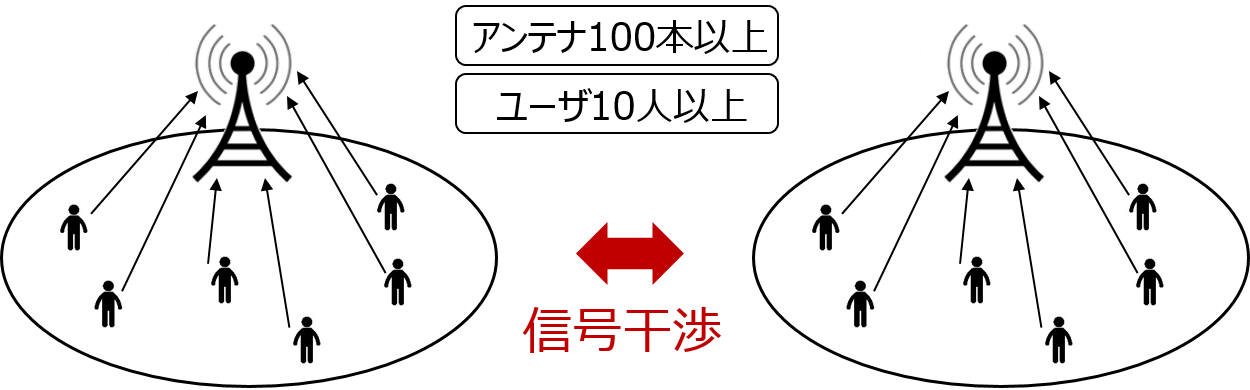
\includegraphics[width=80mm]{./system.png}
    \end{center}
    \caption{想定するシステム}
    \label{fig:system}
\end{figure}

\begin{equation} 
    \label{eq:SendSignal}
	\boldsymbol{X} =  \left(
		\begin{array}{cccc}
			\boldsymbol{X}_{11} &\boldsymbol{X}_{12} &\boldsymbol{P}\\
			\boldsymbol{P} &\boldsymbol{X}_{21} &\boldsymbol{X}_{22}
		\end{array}
	\right).
\end{equation}
樺島AMPアルゴリムの収束性にまだまだ問題があり,前年度までの研究では,パイロット信号$Tp$がユーザ数$K$の倍以上存在しなければ解が発散し,また推定値が振動する問題が発生した.

本年度では,分散の初期値を変更し,ダンピング\cite{vila}によって$Tp=K$でも解を収束することができた.具体的には,初回の通信路推定にて,データ推定の分散を0で初期化し,ダンピング係数を$0.5$にすることで解を収束させた.

さらに,基地局間の距離を考慮し,各ユーザに電力の差異を考慮した場合のシミュレーションを行った.基地局間電力差を2倍にして数値シミュレーションを行った結果,はじめの反復の時は電力差がある場合の結果が通信路推定,BERともに優れていたが,最終的な結果としては反復を繰り返すと,基地局間電力差がない結果と比較してがBERでは$40\%$通信路推定のMSEでは$18\%$悪化している.

また,データのスパース性を高めて推定値の向上を図った.結果として,データの伝送
レートを0.1にしたところ,BERでは$99\%$向上し,通信路推定のMSEでは$87\%$悪化していた.つまり,データ推定の精度は向上するが,通信路推定が犠牲になる.

なお,上記の結果のシミュレーション条件はアンテナ数$N=128$,ユーザ数$K=32$,観測時間$T=128$,パイロット長$Tp=32$であり,反復回数は通信路推定,データ推定をそれぞれ10回ずつ反復し,この二つの推定を合計10回行っている.BERの比較を図に示す.

初回の反復にて分散の初期値を0にすることで推定値が向上する理由として,データ推定を行っていない状態では,未知のデータが通信路推定を妨げるため,分散を0にすることでパイロット信号のみで通信路を推定を行うことで解が収束したと考えられる.また,初回のデータ推定では,パイロット信号を非同期にすることで干渉をうまく計算できないため,通信路の分散を0にすることで解が改善した.また,電力差が生じたときに最終的な結果が悪くなる理由としては,電力差がない場合に比べて,データの電力が小さくなり,通信路推定の結果が低下するため最終的な結果が悪くなる.しかし,電力差が完全に無い場合と比較するにはまだ検討の余地がある.スパース性を高めた場合も同様に,BERの面では利点があるように見受けられるが,送信レートは低くなっているため,比較にはまだ検討が必要である.

\bibliographystyle{ieeetr}
\bibliography{reference}
\end{document}

% end of file
